\section{Architecture}
This chapter describes the architecture of the URL-Archiver. 

\subsection{Frontend}
The frontend architecture of the URL-Archiver is centered on a console-based interface, as evidenced by the \texttt{ConsoleView} and \texttt{CLIController} classes featured in Figure \ref{fig:MVC_Highlevel}.

The \texttt{ConsoleView} class is essential for presenting information and managing user input in a console setting. It is specifically designed to display data and messages clearly and in a user-friendly way. In parallel, the \texttt{CLIController}, a key component of the Controller segment in the MVC (Model-View-Controller) \index{Model-View-Controller (MVC) pattern} framework, serves as an intermediary between the \texttt{ConsoleView} and the application’s backend. This class efficiently processes user inputs from the \texttt{ConsoleView}, interacts with the model to retrieve or modify data, and then updates the console interface with these changes. This architecture is designed to provide efficient and effective user interaction within a command line environment. The Figure \ref{fig:Screenshot_ConsoleView} illustrates the welcome message that the URL archiver displays to users.
%\vskip 0.5cm
\begin{figure}[h!]
    \center
    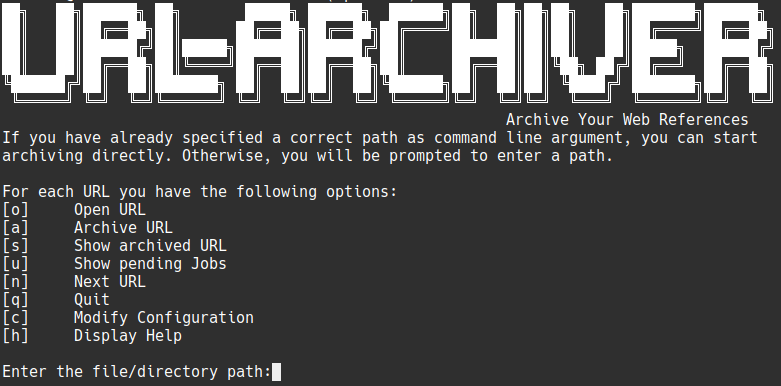
\includegraphics[width=0.9\textwidth]{pictures/final_presentation/command_line_application.jpg}
    \caption{Screenshot of the Console View}
    \label{fig:Screenshot_ConsoleView}
\end{figure}


\subsection{Backend}

\subsubsection{Software Architectural Design}
The URL-Archiver is developed following the principles of the MVC (Model-View-Controller) \index{Model-View-Controller (MVC) pattern} software architectural pattern. The MVC framework \index{Model-View-Controller (MVC) pattern}, as detailed in Figure \ref{fig:MVC_Highlevel}, is a structured approach to building user interfaces in software applications. It organizes an application into three interrelated components:

\begin{itemize}
	\item \textbf{Model:} This layer embodies the URL-Archiver's data structures, business logic, and operational rules. Components such as \texttt{FileModel}, \texttt{FolderModel}, \texttt{URLPair}, and \texttt{ConfigModel}, as shown in Figure \ref{fig:MVC_Highlevel}, represent the model.
	\item \textbf{View:} Tasked with rendering data from the model to the user and forwarding user commands to the controller. The \texttt{ConsoleView} in Figure \ref{fig:MVC_Highlevel} serves as a demonstration of this component.
	\item \textbf{Controller:} It is responsible for handling user inputs, engaging with the model to process data, and selecting the appropriate view for presentation. The \texttt{CLIController}, depicted in Figure \ref{fig:MVC_Highlevel}, is indicative of this segment.
\end{itemize}

This modular structure allows for an efficient separation of code, which aids in easier maintenance and streamlined development. The \texttt{Main} class operates as the launching point for the URL-Archiver, effectively coordinating the MVC pattern \index{Model-View-Controller (MVC) pattern}. Interaction between the Controller and the Model results in updates to the Model, with the View being refreshed in tandem to maintain a clear demarcation of responsibilities.

\begin{figure}[h!]
    \center
    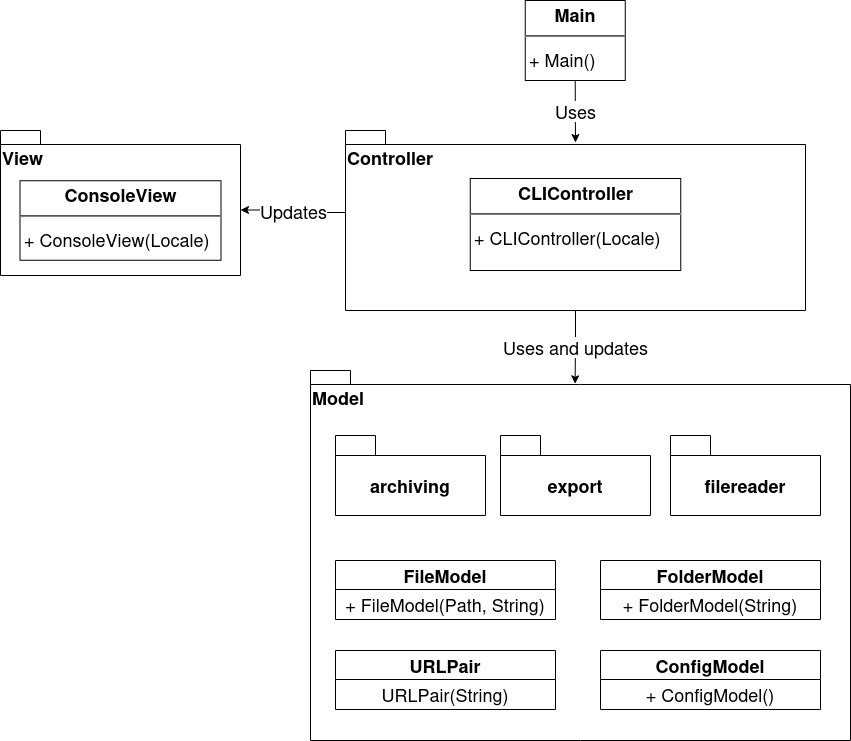
\includegraphics[width=0.65\textwidth]{diagrams/mvc_diagram-Highlevel_MVC.png}
    \caption{Highlevel Diagram of implemented MVC Pattern \index{Model-View-Controller (MVC) pattern}}
    \label{fig:MVC_Highlevel}
\end{figure}
\clearpage

\subsubsection{Factory Pattern}
The URL-Archiver makes extensive use of the Factory Pattern \index{Factory Pattern} in its architecture, a key strategy in software engineering recognised for its role in the creational design paradigm. This pattern is central to the encapsulation of the object instantiation process. Rather than creating objects directly using the "new" operator, the Factory Pattern \index{Factory Pattern} specifies a factory for this purpose. This abstraction improves the flexibility and scalability of the code.

The factory pattern is particularly useful when dealing with a variety of object types to be created, or when specific logic is required in their creation. Its implementation in the URL Archive provides a clear separation of concerns and improves code reusability, in line with the core principles of object-oriented design and programming.

In the URL-Archiver, the Factory Pattern \index{Factory Pattern} is implemented in several key areas:

\begin{itemize}
	\item \textbf{File Readers:} Streamlines the addition of more input file types, thanks to its capability to produce objects conforming to the \texttt{FileReaderInterface}. This factory is pivotal in handling diverse file types.
	\item \textbf{Archiving Services\index{Archiving Services}:} Adding an additional service is straightforward, enhancing the application's ability to integrate different web archiving services.
	\item \textbf{Selenium Web Drivers\index{Selenium}:} Supports the integration of additional browsers with ease, showcasing the pattern’s adaptability in browser interactions.
	\item \textbf{Export Functionality\index{Export Functionality}:} The pattern's application here simplifies the inclusion of support for various file types in the export functionality.
\end{itemize}

These factories contribute significantly to the modularity and extensibility of the URL Archive by encapsulating the creation logic of various components, thus promoting loose coupling and scalability. The alignment of these approaches with the principles of the Factory Design Pattern underscores the maintainability of the application and its adaptability to new file types and data export formats.

The application of the factory pattern in the URL Archive is illustrated in figures \ref{fig:FileReaderFactory_Diagram} and \ref{fig:ExporterFactory_Diagram}, which show the \texttt{FileReaderFactory} and \texttt{ExporterFactory} respectively. Similar design principles are applied to other factories within the application, ensuring a consistent and modular approach across all components.

\begin{figure}[h!]
    \center
    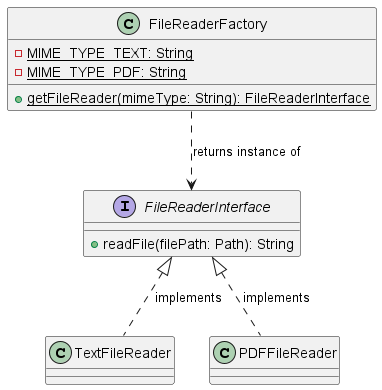
\includegraphics[width=0.5\textwidth]{pictures/FileReaderFactory-0.png}
    \caption{Diagram of the FileReader Factory}
    \label{fig:FileReaderFactory_Diagram}
\end{figure}

\begin{figure}[h!]
    \center
    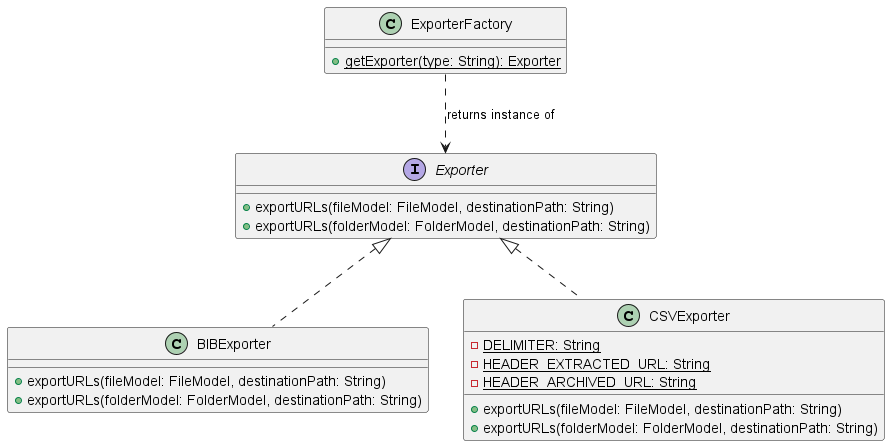
\includegraphics[width=0.9\textwidth]{pictures/ExporterFactory-0.png}
    \caption{Diagram of the Exporter Factory}
    \label{fig:ExporterFactory_Diagram}
\end{figure}
\clearpage

\subsubsection{Configuration File Management}
The URL-Archiver uses a JSON configuration file \index{Configuration File} to effectively manage various settings and parameters. Key classes such as \texttt{ConfigModel} and \texttt{ConfigFileHelper} are integral to this process. The \texttt{ConfigModel} is used to define the structure of the configuration data, ensuring that all essential settings are systematically represented and easily accessible within the application. Conversely, the ConfigFileHelper is responsible for reading and writing the JSON configuration file \index{Configuration File}, decoupling these tasks from the rest of the application code. This methodology not only streamlines the management of configuration settings, but also increases the adaptability of the application, as configuration changes do not require codebase changes.

An example of the configuration file \index{Configuration File} structure is as follows:

\{

\quad''accessKey'':''[Access Key]'',

\quad''secretKey'':''[Secretkey]'',

\quad''browser'':''FIREFOX''

\}

Users have the flexibility to modify the configuration file \index{Configuration File} at runtime, or edit the file directly. Currently, the application uses this file to store credentials for the Wayback Machine and to select the correct browser for the Archive Today service. This feature underlines the URL-Archiver's commitment to user customisation and operational efficiency.
\clearpage
\subsubsection{Adherence to SOLID Principles}
The URL-Archiver has been carefully designed with a strong emphasis on SOLID principles\index{SOLID Principles}, ensuring a robust, maintainable and scalable architecture.

\begin{enumerate}
	\item \textbf{Single Responsibility Principle:} Each class, such as \texttt{FileReaderFactory}, \texttt{ConfigModel} or \texttt{CLIController}, is dedicated to a single responsibility. This principle ensures that each module or class focuses on a single aspect of the application's functionality.
	\item \textbf{Open/Closed Principle:} The application uses interfaces such as \texttt{FileReaderInterface} and factory classes to facilitate extensibility while keeping changes to existing code to a minimum. This approach allows new functionality to be added seamlessly.
	\item \textbf{Liskov Substitution Principle:} The architectural design allows subclasses (such as specific file readers) to replace their parent class or interface without compromising the integrity of the application, thereby maintaining a robust design.
	\item \textbf{Interface separation principle:} The design strategy of the URL Archive favours lean interfaces, ensuring that classes implement only the methods essential to their functionality. This is evident in the focused methods of interfaces such as \texttt{URLArchiver} and \texttt{Exporter}.
	\item \textbf{Dependency Inversion Principle:} High-level modules such as \texttt{CLIController} rely on abstractions rather than concrete implementations. This is emphasised by the use of interfaces and factory classes for object creation, which reduces dependency on specific implementations.
\end{enumerate}

The URL-Archiver's strict adherence to these SOLID principles \index{SOLID Principles} is a testament to its well-structured, easily maintainable and scalable design. This approach underlines the application's commitment to high quality software engineering practices.
\newgeometry{bottom=1cm} % sets the left margin to 1cm
\begin{landscape}
	\thispagestyle{empty}
	\subsubsection{Class Diagram}
	Figure \ref{fig:class_diagram} shows the complete class diagram of our application. A higher resolution version can be found in the appendix, see \ref{app:class_diagram}) (it can be downloaded via double click). 
	\begin{figure}[h!]
		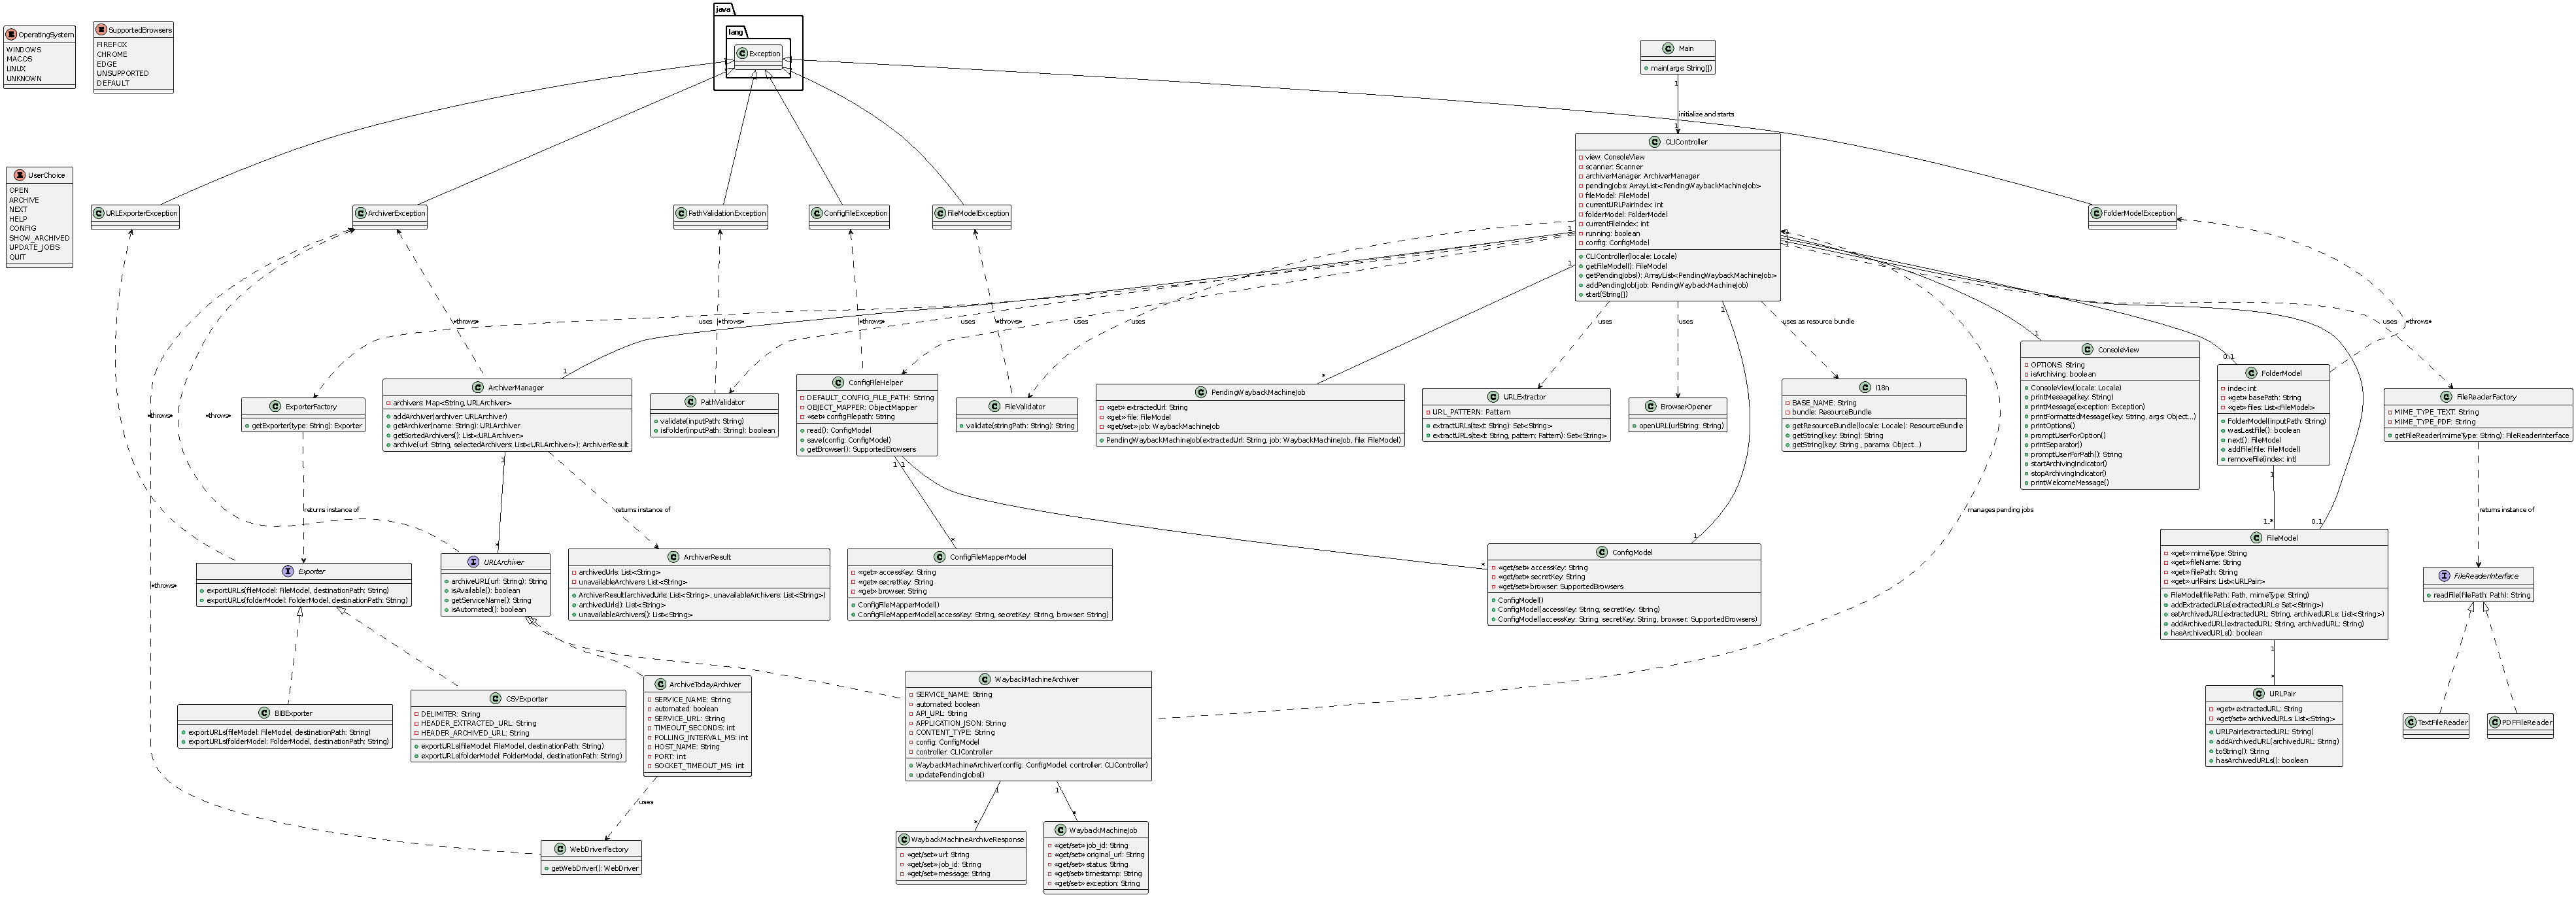
\includegraphics[width=1.9\textwidth]{./diagrams/class_diagram.pdf}
		\centering
		\caption{Class Diagram}
		\label{fig:class_diagram}
	\end{figure}

\end{landscape}
\restoregeometry

\subsection{URL Extraction Process}

The extraction of URLs is a crucial aspect of the architecture, as it determines the effectiveness and accuracy of the archiving system. This description outlines the current approach to URL extraction and identifies areas for improvement.

\subsubsection{URL Extraction Mechanism}
The URL extraction process in the URL-Archiver involves scanning the text content of files and identifying strings that conform to the standard structure of URLs using regular expressions (\gls{regex}) \index{regex}. This technique is essential for processing and archiving the URLs contained within the documents.

\subsubsection{Challenges and Limitations}
The current implementation of the URL extractor, which uses regex\index{regex}, struggles to accurately identify certain types of URLs. One particular challenge is URLs that end with text enclosed in parentheses "()". This issue exposes a limitation in the regex\index{regex} pattern's ability to handle complex URL structures. Detecting URLs through regex\index{regex} is a well-known challenge in the field. This is evidenced by the collection found at Mathias Bynens' "In search of the perfect URL validation regex"\index{regex} \cite{bynens2024urlregex}.

The project's time constraints prevented the development of a more optimized regex pattern to address these specific cases. However, this limitation has been acknowledged as an area for future improvement. Enhancing the regex would significantly improve the URL-Archiver's functionality, making it more robust in handling diverse URL formats.

Furthermore, since it is nearly impossible to achieve perfect URL detection through automated means alone, it is recommended to include a feature that allows users to manually modify the extracted URLs within the URL-Archiver. This functionality would add an extra layer of accuracy, enabling users to correct any errors in URL extraction and ensuring the integrity of the archived data.

